\documentclass[11pt,letterpaper]{article}
\usepackage[margin=1in]{geometry}
\usepackage{amsmath,amssymb,amsthm}
\usepackage{booktabs}
\usepackage{xcolor}
\usepackage{tikz}
\usetikzlibrary{arrows.meta,positioning,calc}
\usepackage{hyperref}
\usepackage{microtype}
\usepackage{enumitem}
\usepackage{fancyhdr}
\usepackage[T1]{fontenc}
\usepackage{lmodern}
\usepackage{colortbl}
\usepackage{tcolorbox}
\usepackage{float}

% ── Colours ──
\definecolor{navy}{HTML}{1b2a4a}
\definecolor{steel}{HTML}{3d5a80}
\definecolor{tint}{HTML}{eef1f6}
\definecolor{wingreen}{HTML}{dceee2}
\definecolor{ruleblue}{HTML}{8a9ab5}
\definecolor{exbg}{HTML}{fff8e7}
\definecolor{defbg}{HTML}{eef6ee}

% ── Theorem environments ──
\theoremstyle{definition}
\newtheorem{definition}{Definition}[section]
\newtheorem{example}{Example}[section]
\newtheorem{remark}{Remark}[section]

% ── tcolorbox styles ──
\tcbset{
  exbox/.style={colback=exbg, colframe=orange!70!black, fonttitle=\bfseries,
                title={Example}, boxrule=0.5pt, arc=2pt, left=4pt, right=4pt, top=2pt, bottom=2pt},
  defbox/.style={colback=defbg, colframe=green!50!black, fonttitle=\bfseries,
                 boxrule=0.5pt, arc=2pt, left=4pt, right=4pt, top=2pt, bottom=2pt},
  keybox/.style={colback=tint, colframe=steel, fonttitle=\bfseries,
                 title={Key Idea}, boxrule=0.5pt, arc=2pt, left=4pt, right=4pt, top=2pt, bottom=2pt},
}

% ── Page style ──
\pagestyle{fancy}
\fancyhf{}
\fancyhead[L]{\small\color{steel} MOLLI: Mathematical Details}
\fancyhead[R]{\small\color{steel} Course Notes}
\fancyfoot[C]{\small\thepage}
\renewcommand{\headrulewidth}{0.4pt}
\renewcommand{\footrulewidth}{0.4pt}

\setlength{\parindent}{0pt}
\setlength{\parskip}{6pt}

\begin{document}

% ══════════════════════════════════════════════════════════════
%  TITLE
% ══════════════════════════════════════════════════════════════
\begin{center}
{\LARGE\bfseries\color{navy} MOLLI: Model Optimization via Likelihood-based Introgression}\\[8pt]
{\large\color{steel} Mathematical Details and Worked Examples}\\[4pt]
{\normalsize Course Notes for the Bayesian Gene Scoring Procedure}
\end{center}
\vspace{4pt}
{\color{navy}\hrule height 0.5pt}
\vspace{12pt}

\tableofcontents
\vspace{12pt}

% ══════════════════════════════════════════════════════════════
\section{Mathematical Preliminaries}
% ══════════════════════════════════════════════════════════════

Before describing the MOLLI algorithm, we review several concepts from probability and calculus that the method relies on. Readers comfortable with Bayesian statistics and gradients may skip to Section~\ref{sec:method}.

\subsection{Random Variables and Variance}

A \textbf{random variable} $X$ is a quantity whose value is determined by a random process. For example, if we roll a die, the outcome $X$ could be any integer from 1 to 6.

The \textbf{expected value} (or mean) of $X$ is the average value we would observe over many repetitions:
\[
\mathbb{E}[X] = \mu = \sum_x x \cdot P(X = x)
\]
For continuous variables, the sum becomes an integral.

The \textbf{variance} measures how spread out the values of $X$ are around the mean:
\[
\text{Var}(X) = \mathbb{E}\bigl[(X - \mu)^2\bigr] = \mathbb{E}[X^2] - \mu^2
\]
A small variance means $X$ tends to be close to $\mu$; a large variance means $X$ is often far from $\mu$. The \textbf{standard deviation} is $\sigma = \sqrt{\text{Var}(X)}$, which has the same units as $X$.

\begin{tcolorbox}[exbox]
If $X$ represents the height of randomly chosen adults (in cm), we might have $\mu = 170$ and $\sigma = 10$. This means most people are within about 10\,cm of 170\,cm.
\end{tcolorbox}

\subsection{The Normal (Gaussian) Distribution}

The \textbf{normal distribution} $\mathcal{N}(\mu, \sigma^2)$ is a bell-shaped distribution parameterized by its mean $\mu$ and variance $\sigma^2$. Its probability density function is:
\[
f(x) = \frac{1}{\sqrt{2\pi\sigma^2}} \exp\!\left(-\frac{(x - \mu)^2}{2\sigma^2}\right)
\]

Key properties:
\begin{itemize}[nosep]
  \item About 68\% of values fall within $\pm 1\sigma$ of the mean.
  \item About 95\% fall within $\pm 2\sigma$.
  \item The \textbf{cumulative distribution function} (CDF), written $\Phi(z)$ for the standard normal $\mathcal{N}(0,1)$, gives the probability that a draw is $\leq z$:
  \[
  \Phi(z) = P(Z \leq z) = \int_{-\infty}^{z} \frac{1}{\sqrt{2\pi}} e^{-t^2/2}\, dt
  \]
  \item Therefore, $P(Z > z) = 1 - \Phi(z)$.
\end{itemize}

\begin{tcolorbox}[exbox]
If $Z \sim \mathcal{N}(0,1)$, then $P(Z > 0) = 1 - \Phi(0) = 0.5$ (by symmetry). If $Z \sim \mathcal{N}(2, 1)$, then $P(Z > 0) = 1 - \Phi(-2) \approx 0.977$---we are 97.7\% confident $Z$ is positive.
\end{tcolorbox}

\subsection{Bayesian Inference: The Core Idea}

In \textbf{Bayesian inference}, we start with a \emph{prior belief} about some unknown quantity $\theta$, observe data $D$, and update our belief to get a \emph{posterior}:
\[
\underbrace{P(\theta \mid D)}_{\text{posterior}} \;\propto\; \underbrace{P(D \mid \theta)}_{\text{likelihood}} \;\times\; \underbrace{P(\theta)}_{\text{prior}}
\]

In words: what we believe after seeing the data is proportional to how likely the data would be under each possible value of $\theta$, weighted by what we believed before.

\begin{tcolorbox}[keybox]
Bayesian inference lets us combine uncertain measurements with prior knowledge to get better estimates. When data is noisy, the prior ``regularizes'' our estimate, pulling it away from extreme values that are likely due to noise.
\end{tcolorbox}

\subsection{Conjugate Normal Model}

A particularly clean case arises when both the prior and the likelihood are normal distributions. Suppose:
\begin{align}
\text{Prior:} \qquad & \theta \sim \mathcal{N}(\mu_0, \tau^2) \label{eq:prior} \\
\text{Likelihood:} \qquad & X \mid \theta \sim \mathcal{N}(\theta, \sigma^2) \label{eq:lik}
\end{align}

Then the posterior is also normal:
\begin{equation}
\theta \mid X \sim \mathcal{N}\!\left(B \cdot X + (1 - B) \cdot \mu_0, \;\; B \cdot \sigma^2\right)
\label{eq:posterior}
\end{equation}
where the \textbf{shrinkage factor} is:
\begin{equation}
B = \frac{\tau^2}{\tau^2 + \sigma^2}
\label{eq:shrinkage}
\end{equation}

\begin{tcolorbox}[keybox]
The posterior mean is a \textbf{weighted average} of the observed data $X$ and the prior mean $\mu_0$. The weight $B$ depends on the \textbf{signal-to-noise ratio}: when $\tau^2 \gg \sigma^2$ (signal dominates), $B \approx 1$ and we trust the data. When $\sigma^2 \gg \tau^2$ (noise dominates), $B \approx 0$ and we trust the prior.
\end{tcolorbox}

\begin{tcolorbox}[exbox]
Suppose we're estimating a baseball player's true batting average. Our prior is that most players bat around $\mu_0 = 0.260$ with $\tau = 0.03$. We observe a player batting $X = 0.400$ over 10 at-bats, with observation noise $\sigma = 0.15$. Then:
\[
B = \frac{0.03^2}{0.03^2 + 0.15^2} = \frac{0.0009}{0.0234} \approx 0.038
\]
Posterior mean $= 0.038 \times 0.400 + 0.962 \times 0.260 \approx 0.265$.

The small sample gives high noise ($\sigma \gg \tau$), so $B \approx 0$ and we barely trust the observation---our estimate is pulled almost entirely back to the league average. This is \emph{shrinkage} at work.
\end{tcolorbox}

\subsection{Gradients and Partial Derivatives}

A \textbf{gradient} $\nabla_\theta f$ is the vector of partial derivatives of a function $f$ with respect to each element of a vector $\theta$:
\[
\nabla_\theta f = \left(\frac{\partial f}{\partial \theta_1}, \frac{\partial f}{\partial \theta_2}, \ldots, \frac{\partial f}{\partial \theta_d}\right)
\]
Each partial derivative $\frac{\partial f}{\partial \theta_k}$ tells us how much $f$ changes when we change $\theta_k$ by a tiny amount, holding all other parameters fixed.

\subsection{First-Order Taylor Approximation}

For a small change $\Delta\theta$ in the parameter vector, the change in $f$ is approximately:
\begin{equation}
f(\theta + \Delta\theta) - f(\theta) \;\approx\; \sum_{k=1}^d \frac{\partial f}{\partial \theta_k} \cdot \Delta\theta_k \;=\; \nabla_\theta f \cdot \Delta\theta
\label{eq:taylor}
\end{equation}
This linear approximation works well when $\Delta\theta$ is small relative to the scale of $\theta$. It avoids computing $f$ at the perturbed point---we only need the gradient at the original point and the perturbation vector.

\subsection{Perplexity}

\textbf{Perplexity} (PPL) measures how well a language model predicts text. It is defined as:
\[
\text{PPL} = \exp\!\left(\frac{1}{N} \sum_{i=1}^N -\log P(x_i \mid x_1, \ldots, x_{i-1})\right)
\]
where $x_1, \ldots, x_N$ are the tokens in a text and $P(x_i \mid \cdots)$ is the model's predicted probability for token $x_i$. Intuitively:
\begin{itemize}[nosep]
  \item PPL $= 1$: the model predicts every token with certainty.
  \item PPL $= 10$: on average, the model is as uncertain as choosing from 10 equally likely options.
  \item PPL $= 50{,}000$: the model is essentially guessing randomly.
\end{itemize}
\textbf{Lower perplexity is better.} The geometric mean (GM) of perplexities across domains gives a single summary of overall model quality.


% ══════════════════════════════════════════════════════════════
\section{The MOLLI Algorithm}
\label{sec:method}
% ══════════════════════════════════════════════════════════════

\subsection{Setup: Genes and Dual-Strand Encoding}

A neural network has $d$ parameters (weights) $\theta = (\theta_1, \theta_2, \ldots, \theta_d)$. We partition these into $L$ non-overlapping groups called \textbf{genes}:
\[
\theta = (g_1, g_2, \ldots, g_L), \qquad g_i = (\theta_{s_i}, \theta_{s_i + 1}, \ldots, \theta_{e_i})
\]
where $[s_i, e_i]$ is the index range of gene $i$. Each gene corresponds to a functional unit of the network: an attention head, an MLP block, or a normalization layer. For a 7-billion-parameter model, this gives $L = 928$ genes.

We maintain two copies of all parameters:
\begin{itemize}[nosep]
  \item \textbf{Primary strand} $\mathbf{w}^p$: the live, trainable weights (full precision).
  \item \textbf{Complement strand} $\mathbf{w}^c$: a quantized snapshot (int16) of the weights taken before training on the new domain. This represents the ``healthy'' state.
\end{itemize}

\begin{tcolorbox}[defbox, title={Biological Analogy}]
In the Amazon Molly, the two chromosome copies serve the same role: one may acquire a harmful mutation during reproduction, and the other provides a ``backup'' to repair it. In MOLLI, fine-tuning introduces ``mutations'' (weight changes), and the complement strand is the backup.
\end{tcolorbox}

\subsection{The Evolution Cycle}

For each new domain $k$ in the sequence, MOLLI executes five steps:

\begin{center}
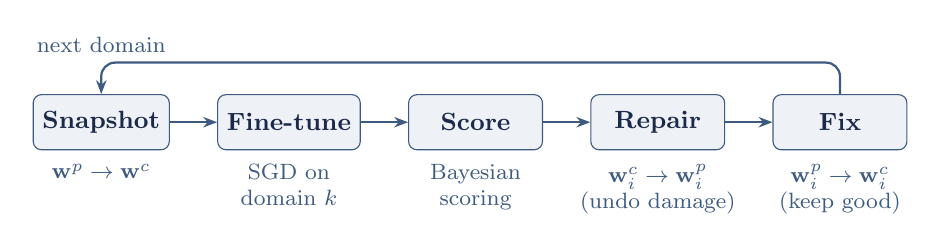
\begin{tikzpicture}[
  node distance=0.3cm and 0.6cm,
  box/.style={rectangle, rounded corners=3pt, draw=steel, fill=tint,
              minimum height=0.7cm, minimum width=1.7cm,
              font=\small\bfseries, text=navy, align=center},
  arr/.style={-{Stealth[length=5pt]}, thick, color=steel},
  lbl/.style={font=\footnotesize\color{steel}, align=center},
]
  \node[box](s){\small Snapshot}; \node[box,right=of s](t){\small Fine-tune};
  \node[box,right=of t](sc){\small Score}; \node[box,right=of sc](r){\small Repair};
  \node[box,right=of r](f){\small Fix};
  \draw[arr](s)--(t); \draw[arr](t)--(sc); \draw[arr](sc)--(r); \draw[arr](r)--(f);
  \draw[arr,rounded corners=5pt](f.north)--++(0,0.4)-|node[above,pos=0.5,lbl]{next domain}(s.north);
  \node[lbl,below=0.05 of s]{$\mathbf{w}^p \to \mathbf{w}^c$};
  \node[lbl,below=0.05 of t]{SGD on\\domain $k$};
  \node[lbl,below=0.05 of sc]{Bayesian\\scoring};
  \node[lbl,below=0.05 of r]{$\mathbf{w}^c_i \to \mathbf{w}^p_i$\\(undo damage)};
  \node[lbl,below=0.05 of f]{$\mathbf{w}^p_i \to \mathbf{w}^c_i$\\(keep good)};
\end{tikzpicture}
\end{center}

\textbf{Step 1: Snapshot.} Quantize the current primary weights into the complement strand: $\mathbf{w}^c \leftarrow \text{quantize}(\mathbf{w}^p)$. After this, $\mathbf{w}^c$ represents the pre-training state.

\textbf{Step 2: Fine-tune.} Train the primary weights $\mathbf{w}^p$ on the new domain $k$ using standard stochastic gradient descent. This changes $\mathbf{w}^p$ but leaves $\mathbf{w}^c$ unchanged. The model now performs well on domain $k$ but may have lost performance on prior domains.

\textbf{Step 3: Score.} For each gene $i$ and each prior domain $j$, estimate how much damage (or benefit) the fine-tuning caused. This is the core mathematical contribution and is detailed in Sections~\ref{sec:scoring}--\ref{sec:bayes}.

\textbf{Step 4: Repair.} Genes identified as damaged are reverted by copying from the complement: $\mathbf{w}^p_i \leftarrow \mathbf{w}^c_i$. See Section~\ref{sec:decision}.

\textbf{Step 5: Fix.} Genes identified as beneficial and harmless to all prior domains have their complement updated: $\mathbf{w}^c_i \leftarrow \mathbf{w}^p_i$, permanently incorporating the adaptation.


% ══════════════════════════════════════════════════════════════
\section{Gene Scoring via Gradient Approximation}
\label{sec:scoring}
% ══════════════════════════════════════════════════════════════

\subsection{The Question We Want to Answer}

After fine-tuning on domain $k$, gene $i$'s weights have changed from $\mathbf{w}^c_i$ (pre-training) to $\mathbf{w}^p_i$ (post-training). For each prior domain $j$, we want to know:

\begin{quote}
\emph{If we reverted gene $i$ back to its pre-training state (replacing $\mathbf{w}^p_i$ with $\mathbf{w}^c_i$), how would the loss on domain $j$ change?}
\end{quote}

Let $\mathcal{L}_j(\theta)$ denote the loss on domain $j$'s evaluation data when the model has parameters $\theta$. After fine-tuning, the current parameters are $\mathbf{w}^p$. If we revert gene $i$, we get a \textbf{chimeric} parameter vector $\tilde{\theta}$ that is identical to $\mathbf{w}^p$ except for gene $i$:
\[
\tilde{\theta}_k = \begin{cases} w^c_k & \text{if } k \in g_i \\ w^p_k & \text{otherwise} \end{cases}
\]

The exact reversion effect is $\mathcal{L}_j(\tilde{\theta}) - \mathcal{L}_j(\mathbf{w}^p)$, but computing this requires a separate forward pass for each of the $L = 928$ genes and each of the $J$ prior domains---$928 \times J$ forward passes total.

\subsection{The Taylor Approximation}

Instead, we use the first-order Taylor approximation (Eq.~\ref{eq:taylor}). The change from $\mathbf{w}^p$ to $\tilde{\theta}$ only affects the parameters in gene $i$, and the change is $\Delta\theta_k = w^c_k - w^p_k$ for $k \in g_i$ (zero elsewhere). Therefore:

\begin{equation}
\boxed{\delta_{ij} \;=\; \sum_{k \in g_i} \frac{\partial \mathcal{L}_j}{\partial \theta_k}\Bigg|_{\theta = \mathbf{w}^p} \cdot \bigl(w^c_k - w^p_k\bigr)}
\label{eq:genescore}
\end{equation}

This is the \textbf{gene score}: a scalar estimating how much reverting gene $i$ would change the loss on domain $j$.

\begin{itemize}[nosep]
  \item If $\delta_{ij} < 0$: reverting gene $i$ would \emph{decrease} the loss on domain $j$ (repairing would help---the gene was \emph{damaged} by training).
  \item If $\delta_{ij} > 0$: reverting would \emph{increase} the loss (the gene's changes actually \emph{benefit} domain $j$).
  \item If $\delta_{ij} \approx 0$: the gene's changes had negligible effect on domain $j$.
\end{itemize}

\begin{tcolorbox}[keybox]
The crucial efficiency insight: the gradient $\frac{\partial \mathcal{L}_j}{\partial \theta_k}$ for \emph{all} $d$ parameters is computed by a single forward+backward pass (backpropagation). Once we have this gradient vector, we extract each gene's score by slicing out the relevant parameters and computing the dot product with the weight change. Total cost: one forward+backward pass per prior domain, yielding \emph{all} gene scores simultaneously.
\end{tcolorbox}

\begin{tcolorbox}[exbox]
Suppose gene $i$ consists of 3 parameters with:
\begin{itemize}[nosep]
  \item Gradients: $\frac{\partial \mathcal{L}_j}{\partial \theta_k} = (0.5, -0.3, 0.1)$
  \item Weight changes: $w^c_k - w^p_k = (-0.2, 0.4, -0.1)$
\end{itemize}
Then $\delta_{ij} = (0.5)(-0.2) + (-0.3)(0.4) + (0.1)(-0.1) = -0.1 - 0.12 - 0.01 = -0.23$.

Since $\delta_{ij} < 0$, reverting this gene would decrease the loss on domain $j$ by approximately 0.23. This gene was \emph{damaged} by fine-tuning and is a repair candidate.
\end{tcolorbox}

\textbf{Sign convention in the code.} In the implementation, the raw score is computed as Eq.~\ref{eq:genescore}. When assessing whether a gene is deleterious, the scores are \emph{negated}: we define $d_{ij} = -\delta_{ij}$, so that positive $d_{ij}$ means ``repairing helps'' (the gene is deleterious). The Bayesian analysis is performed on these negated scores.


% ══════════════════════════════════════════════════════════════
\section{Split-Half Noise Estimation}
\label{sec:splithalf}
% ══════════════════════════════════════════════════════════════

\subsection{Why We Need Noise Estimation}

The gene score $\delta_{ij}$ from Eq.~\ref{eq:genescore} is computed using a finite set of evaluation samples. If we used a different random subset, we would get a slightly different score. This randomness is \textbf{observation noise}.

Some genes might have $\delta_{ij} = -0.23$ purely by chance, even if the true effect is zero. If we repair every gene with a negative score, we would be making many false-positive repairs---reverting genes that weren't actually damaged. We need to estimate how noisy the scores are.

\subsection{The Split-Half Procedure}

Given $N$ evaluation samples, we split them into two halves (A and B), each of size $N/2$:
\begin{align}
\delta^A_{ij} &= \text{gene score using samples from half A} \\
\delta^B_{ij} &= \text{gene score using samples from half B}
\end{align}

The combined score is the average: $\delta_{ij} = (\delta^A_{ij} + \delta^B_{ij}) / 2$.

\textbf{Estimating noise variance.} Each half-score has some noise variance $\sigma^2_\text{half}$. The difference $\delta^A - \delta^B$ has variance $2\sigma^2_\text{half}$ (since the halves are independent). The combined average $(\delta^A + \delta^B)/2$ has variance $\sigma^2_\text{half}/2$. Therefore:
\begin{equation}
\sigma^2 = \frac{\text{Var}(\delta^A - \delta^B)}{4}
\label{eq:noisevar}
\end{equation}
where the variance is taken across genes (treating $\delta^A_i - \delta^B_i$ for $i = 1, \ldots, L$ as a sample).

\textbf{Split-half correlation.} As a diagnostic, we also compute the Pearson correlation between $\delta^A$ and $\delta^B$ across genes. High correlation ($r \approx 1$) indicates the scores are reliable and reproducible; low correlation indicates noise dominance. In our experiments, $r$ ranged from $0.83$ to $0.999$.

\begin{tcolorbox}[exbox]
With 49 evaluation samples, we use 24 for half A and 24 for half B (dropping 1). Suppose across 928 genes, we compute $\delta^A_i$ and $\delta^B_i$ for each. The differences $\delta^A_i - \delta^B_i$ have variance $0.0012$. Then $\sigma^2 = 0.0012 / 4 = 0.0003$, and $\sigma = 0.017$.

If the overall variance of $\delta_i$ is $0.005$, the signal-to-noise ratio is $(0.005 - 0.0003) / 0.0003 \approx 15.7$---plenty of signal.
\end{tcolorbox}


% ══════════════════════════════════════════════════════════════
\section{Empirical Bayes Shrinkage}
\label{sec:bayes}
% ══════════════════════════════════════════════════════════════

\subsection{The Generative Model}

We now have, for each gene $i$ and prior domain $j$:
\begin{itemize}[nosep]
  \item An observed score $d_{ij}$ (the negated combined score).
  \item An estimate of its noise variance $\sigma^2$ (from split-half).
\end{itemize}

We model the scores across genes using the conjugate normal model from Section~1.4:
\begin{align}
\text{Prior (true gene effects):} \qquad & \mu_i \sim \mathcal{N}(\mu_0, \tau^2) \label{eq:molli_prior}\\
\text{Likelihood (noisy observation):} \qquad & d_i \mid \mu_i \sim \mathcal{N}(\mu_i, \sigma^2) \label{eq:molli_lik}
\end{align}

Here $\mu_i$ is the \emph{true} effect of reverting gene $i$ (unknown), and $d_i$ is the noisy observed score. The prior says that most genes have effects near $\mu_0$ (the population mean), with spread $\tau^2$.

\subsection{Estimating the Parameters (Method of Moments)}

The model has three unknown parameters: $\mu_0$, $\tau^2$, and $\sigma^2$. We estimate them from data:

\textbf{Noise variance $\sigma^2$:} Already estimated from split-half (Eq.~\ref{eq:noisevar}).

\textbf{Prior mean $\mu_0$:} Estimated as the sample mean of all gene scores:
\[
\hat{\mu}_0 = \frac{1}{L} \sum_{i=1}^L d_i
\]

\textbf{Signal variance $\tau^2$ (method of moments):} The total observed variance across genes is:
\[
\text{Var}(d) = \frac{1}{L} \sum_{i=1}^L (d_i - \hat{\mu}_0)^2
\]
Under our model, $\text{Var}(d) = \tau^2 + \sigma^2$ (the observed spread is the sum of true variation plus noise). Therefore:
\begin{equation}
\hat{\tau}^2 = \max\!\bigl(0, \;\text{Var}(d) - \sigma^2\bigr)
\label{eq:tau2}
\end{equation}
The $\max(0, \cdot)$ ensures we don't get a negative variance estimate (which would happen when noise exceeds total variance---meaning there is essentially no signal).

\subsection{Computing the Posterior}

Using the conjugate formula (Eq.~\ref{eq:posterior}):

\begin{equation}
\boxed{B = \frac{\hat{\tau}^2}{\hat{\tau}^2 + \sigma^2}, \qquad \delta^*_i = B \cdot d_i + (1 - B) \cdot \hat{\mu}_0, \qquad \text{Var}_\text{post} = B \cdot \sigma^2}
\label{eq:molli_posterior}
\end{equation}

\begin{tcolorbox}[keybox]
The shrinkage factor $B$ is the same for all genes within one objective. It acts as a \textbf{global confidence dial}: when the objective's gene scores are mostly signal ($B \approx 1$), we trust individual scores; when mostly noise ($B \approx 0$), every gene's score is pulled toward the mean, preventing false positives.
\end{tcolorbox}

\begin{tcolorbox}[exbox, title={Worked Example: Shrinkage in Action}]
Consider scoring 928 genes for the ``code'' domain. Suppose:
\begin{itemize}[nosep]
  \item Observed gene scores: mean $\hat{\mu}_0 = 0.001$, variance $\text{Var}(d) = 0.005$
  \item Noise variance from split-half: $\sigma^2 = 0.0003$
\end{itemize}

Signal variance: $\hat{\tau}^2 = 0.005 - 0.0003 = 0.0047$.

Shrinkage: $B = 0.0047 / (0.0047 + 0.0003) = 0.94$.

This means we trust the observed scores 94\% of the way. For a gene with observed score $d_i = 0.05$:
\[
\delta^*_i = 0.94 \times 0.05 + 0.06 \times 0.001 = 0.047
\]
Barely any shrinkage---the score is reliable.

Now suppose a different objective where $\text{Var}(d) = 0.0004$ and $\sigma^2 = 0.0003$. Then $\hat{\tau}^2 = 0.0001$ and $B = 0.0001/0.0004 = 0.25$. For the same gene:
\[
\delta^*_i = 0.25 \times 0.05 + 0.75 \times 0.001 = 0.013
\]
Heavy shrinkage---the score dropped from 0.05 to 0.013 because the objective's scores are too noisy to trust.
\end{tcolorbox}

\subsection{Computing Posterior Probabilities}

The posterior distribution for gene $i$'s true effect is:
\[
\mu_i \mid d_i \sim \mathcal{N}(\delta^*_i, \;\text{Var}_\text{post})
\]

The probability that gene $i$ is truly deleterious (i.e., repairing it would help) is the probability that the true effect is positive:
\begin{equation}
\boxed{P(\text{del}_i) = P(\mu_i > 0 \mid d_i) = 1 - \Phi\!\left(\frac{-\delta^*_i}{\sqrt{\text{Var}_\text{post}}}\right)}
\label{eq:pdel}
\end{equation}

This is a \textbf{calibrated probability}: it accounts for observation noise and corrects for multiple testing across genes.

\begin{tcolorbox}[exbox]
Continuing from above ($B = 0.94$), with $\delta^*_i = 0.047$ and $\text{Var}_\text{post} = 0.94 \times 0.0003 = 0.000282$, so $\sqrt{\text{Var}_\text{post}} = 0.0168$:
\[
P(\text{del}_i) = 1 - \Phi\!\left(\frac{-0.047}{0.0168}\right) = 1 - \Phi(-2.80) = 0.997
\]
We are 99.7\% confident this gene is deleterious---strong evidence for repair.

For the noisy objective ($B = 0.25$), $\delta^*_i = 0.013$, $\text{Var}_\text{post} = 0.25 \times 0.0003 = 0.000075$, $\sqrt{\text{Var}_\text{post}} = 0.0087$:
\[
P(\text{del}_i) = 1 - \Phi(-0.013/0.0087) = 1 - \Phi(-1.49) = 0.932
\]
Still fairly confident (93.2\%), but less so. The shrinkage appropriately reduced our certainty.
\end{tcolorbox}


% ══════════════════════════════════════════════════════════════
\section{The Repair Decision}
\label{sec:decision}
% ══════════════════════════════════════════════════════════════

\subsection{Multi-Objective Aggregation}

The scoring procedure yields $P(\text{del}_{ij})$ for each gene $i$ and prior domain $j$, plus $P(\text{ben}_i)$ for the current domain (computed analogously, using the raw---not negated---scores). To make a single repair decision per gene, we aggregate across domains by taking the \textbf{maximum} deleterious probability:
\[
P_{\max}(i) = \max_{j \in \text{prior domains}} P(\text{del}_{ij})
\]
This conservative strategy means a gene is flagged for repair if it damages \emph{any} prior domain, even if it's fine for others.

\subsection{The Trade-off Score}

Repairing a gene undoes damage to prior domains but may also remove benefit to the current domain. The \textbf{trade score} balances these:
\begin{equation}
\text{trade}_i = P_{\max}(i) - \alpha \cdot P(\text{ben}_i)
\label{eq:trade}
\end{equation}
where $\alpha \in [0, 1]$ controls how much we value current-domain benefit relative to prior-domain protection. In our experiments, $\alpha = 0.3$.

\subsection{Decision Rules}

\textbf{Repair:} Gene $i$ is a repair candidate if $\text{trade}_i > \theta$ (threshold, default $\theta = 0.8$). All candidates are ranked by trade score (highest = most damaged), and at most $p\%$ of genes are repaired per cycle ($p = 15\%$ in our experiments, i.e., 139 out of 928 genes).

\textbf{Fix:} Gene $i$ is fixed (complement updated) if $P(\text{del}_{ij}) < 0.3$ for \emph{all} prior domains $j$. This means we are confident the gene's changes are harmless to everything learned so far, so we permanently accept them.

\begin{tcolorbox}[exbox, title={Repair Candidate Selection}]
After training on domain 3 (medical), with 2 prior domains (code, legal):
\begin{center}
\small
\begin{tabular}{@{}lccccp{3.2cm}@{}}
\toprule
Gene & $P_\text{code}$ & $P_\text{legal}$ & $P_\text{max}$ & $P_\text{ben}$ & Decision \\
\midrule
attn\_h3\_L5 & .997 & .42 & .997 & .12 & $.997\!-\!0.3(.12)\!=\!.96$ \textbf{Repair} \\
mlp\_up\_L8 & .15 & .22 & .22 & .85 & $.22\!-\!0.3(.85)\!=\!-.04$ No repair \\
ln\_L2 & .08 & .11 & .11 & .35 & $P_\text{max}\!<\!0.3$: \textbf{Fix} \\
\bottomrule
\end{tabular}
\end{center}

Gene \texttt{attn\_h3\_L5} is strongly deleterious to code (99.7\%) and mildly to legal (42\%), with low benefit to medical (12\%). It gets repaired.

Gene \texttt{mlp\_up\_L8} has low damage but high benefit (85\%)---we keep it.

Gene \texttt{ln\_L2} has very low damage everywhere ($< 0.3$) so we fix it: copy primary $\to$ complement, accepting the adaptation permanently.
\end{tcolorbox}


% ══════════════════════════════════════════════════════════════
\section{Experimental Results}
\label{sec:results}
% ══════════════════════════════════════════════════════════════

All experiments use Qwen2.5-7B (7.6B parameters, $L = 928$ genes), fine-tuned for 3 epochs per domain in bfloat16 with an 8-bit Adam optimizer. Evaluation uses 49 samples of 256 tokens per domain.

\begin{table}[H]
\centering
\caption{Geometric mean perplexity after sequential training (lower is better).}
\label{tab:scaling}
\small
\begin{tabular}{@{}lcccc@{}}
\toprule
\textbf{Domains} & \textbf{MOLLI} & \textbf{LoRA} & \textbf{Impr.} & \textbf{Time (M\,/\,L)} \\
\midrule
3 (code $\to$ legal $\to$ medical) & \textbf{1.60} & 2.10 & $-$24\% & 38\,m / 15\,m \\
\rowcolor{wingreen}
5 (+ science, finance) & \textbf{1.11} & 1.45 & $-$23\% & 113\,m / 49\,m \\
6 (+ general) & \textbf{1.52} & 1.60 & $-$5\% & 146\,m / 62\,m \\
\bottomrule
\end{tabular}
\end{table}

\begin{table}[H]
\centering
\caption{Per-domain perplexity after all sequential training phases.}
\label{tab:perdomain}
\small
\begin{tabular}{@{}lccccccc@{}}
\toprule
& gen & code & legal & med & sci & fin & \textbf{GM} \\
\midrule
\rowcolor{wingreen}
\textbf{MOLLI (5d)} & 1.06 & 1.25 & 1.10 & 1.14 & 1.06 & 1.06 & \textbf{1.11} \\
LoRA (5d) & 1.10 & 1.63 & 1.83 & 2.29 & 1.10 & 1.10 & 1.45 \\
\midrule
\textbf{MOLLI (6d)} & 1.05 & 1.53 & 2.53 & 2.80 & 1.05 & 1.05 & \textbf{1.52} \\
LoRA (6d) & 1.11 & 1.68 & 2.81 & 2.65 & 1.11 & 1.11 & 1.60 \\
\bottomrule
\end{tabular}
\end{table}

\textbf{Interpretation.} At 5 domains, MOLLI retains near-perfect performance on all prior domains (all $\leq 1.25$), while LoRA shows the O(1/N) dilution effect: medical degrades to 2.29 and legal to 1.83. At 6 domains, both methods show some forgetting on middle domains (legal, medical), but MOLLI still maintains a lower overall GM. The narrower gap at 6 domains (5\% vs 23\%) suggests the fixed 15\% repair cap becomes a bottleneck when balancing 7 simultaneous objectives.

\textbf{Scoring reliability.} Split-half correlations ranged from $r = 0.83$ (on noisier objectives like the code domain after medical training) to $r = 0.999$ (on the general domain). Shrinkage factors $B$ ranged from 0.75 (SNR $= 3.1$, conservative shrinkage) to 0.999 (SNR $= 842.5$, minimal shrinkage). In all cases, the empirical Bayes procedure appropriately modulated confidence.

\textbf{Repair statistics.} Exactly 139 genes (the 15\% cap) were repaired in each cycle, and 0--151 genes were fixed per domain. The cap was saturated in every cycle, suggesting that relaxing or adapting it could further improve results.


% ══════════════════════════════════════════════════════════════
\section{Summary}
% ══════════════════════════════════════════════════════════════

The MOLLI algorithm can be summarized in four key ideas:

\begin{enumerate}
  \item \textbf{Dual-strand encoding} provides a healthy reference (the complement) against which to measure fine-tuning damage.
  \item \textbf{Gradient-based gene scoring} (Eq.~\ref{eq:genescore}) efficiently estimates the effect of reverting each gene using a first-order Taylor approximation, requiring only one forward+backward pass per objective.
  \item \textbf{Empirical Bayes shrinkage} (Eqs.~\ref{eq:tau2}--\ref{eq:molli_posterior}) separates signal from noise and produces calibrated posterior probabilities, preventing false-positive repairs.
  \item \textbf{Selective bidirectional repair} (Eq.~\ref{eq:trade}) undoes damage while preserving beneficial changes, mirroring the biological gene conversion mechanism.
\end{enumerate}

The net effect is a continual learning system that actively maintains prior knowledge rather than passively hoping it survives, achieving 23--24\% lower perplexity than LoRA across 3--5 sequential domains.

\end{document}
